\documentclass{report}
\usepackage[letterpaper, margin=1in]{geometry}
\usepackage[utf8]{inputenc}
\usepackage{amsmath}
\usepackage{graphicx}
\usepackage{float}
\usepackage{lscape}
\usepackage{listings}

\setlength{\parindent}{0pt}
\setlength{\parskip}{1em}

\begin{document}

\title{Runtime Effect of Optimization Levels and Compiler Transformations}
\author{Rhea Bhat (rb43853) \\ John Matthew Mason (jmm22836) \\ Eesha Nayak (en5383)}
\maketitle

\section*{Introduction}
Compiler Optimization is a process where the compiler tries to decrease the run time of an application by maximizing program efficiency. To do so, the compiler creates transformations in the code by rearranging sections. There are multiple levels of optimizations starting with the lowest level of -O0 to the highest level of -O3. 

The first level -O0 ensures that the code is run the same way it is written. Starting from -O1, some optimization will occur if possible. The recommended optimization speed is -O2. At the highest -O3 optimization level, higher performance is not guaranteed. Higher performance is only achieved with code that utilizes loop and memory access transformations. The -O3 option is primarily used for programs that have loops that use numerous floating-point calculations and pull large data sets.

\section*{Testing Compiler Optimization}
To figure out the runtimes for each optimization level and each compiler we tested the levels on the given rotate.cxx file. Below are the commands we used to test the run times at four different optimization levels for the Intel and Gnu compilers.

\subsection*{Commands Executed}

We ran each of the following commands and observed the program runtime in the output.  We recorded the results in the table in the following section by compiler and optimization level.

\begin{lstlisting}[language=bash]
login3.frontera(1)$ g++ -O0 rotate.cxx && a.out
login3.frontera(2)$ g++ -O1 rotate.cxx && a.out
login3.frontera(3)$ g++ -O2 rotate.cxx && a.out
login3.frontera(4)$ g++ -O3 rotate.cxx && a.out

login3.frontera(5)$ icc -O0 rotate.cxx && a.out
login3.frontera(6)$ icc -O1 rotate.cxx && a.out
login3.frontera(7)$ icc -O2 rotate.cxx && a.out
login3.frontera(8)$ icc -O3 rotate.cxx && a.out
\end{lstlisting}

\subsection*{Results}

\begin{table}[H]
\centering
\begin{tabular}{|l|l|l|}
\hline
\textbf{Optimization Level} & \textbf{Intel Compiler Runtime} & \textbf{Gnu Compiler Runtime} \\ \hline
0 & 280,530 usec & 427,784 usec \\ \hline
1 & 259,247 usec & 255216 usec \\ \hline
2 & 252,709 usec & 0 usec \\ \hline
3 & 0 usec & 0 usec \\ \hline
\end{tabular}
\caption{Program Runtime Results for Compiler Optimization O0 through O3}
\label{tab:table1}
\end{table}

The runtime clearly decreases as the optimization level increases. Some of the higher optimization levels output 0 usec because the program ran so fast that the runtime was not registered.  
\\At level -O0, no optimization techniques are used. 
\\At level -O1, the code is optimized for size by omitting optimizations that tend to increase object size - this is applicable in situations with large server / databases where memory paging due to large code size is an issue.
\\At level -O2, the code is optimized to maximize speed with tools such as vectorization and intra-file interprocedural optimizations.
\\At level -O3, the -O2 optimization techniques are used with more aggressive loop and memory-access optimizations.

\begin{figure}[H]
\centering
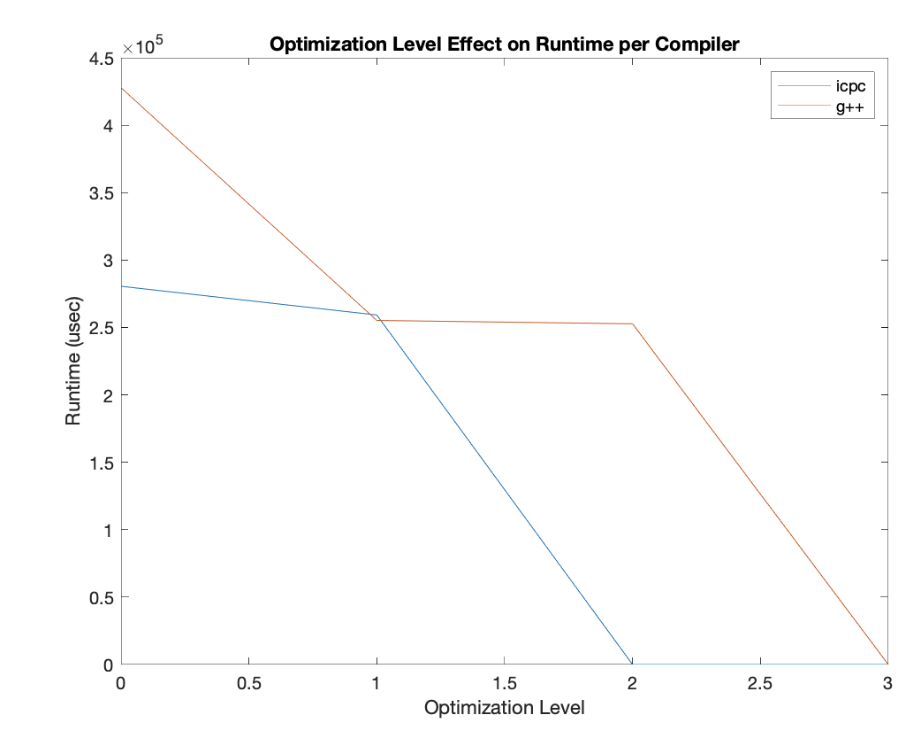
\includegraphics[width=.5\paperwidth]{optimization_graph.png}
\caption{Program Runtime Results for Compiler Optimization O0 through O3}
\end{figure}

\section*{Manual Transformations}
In an attempt to replicate the optimizations used by the compiler, we modified the rotate.cxx file to make it more efficient.  We identified four potential optimizations, adjusted the code, and ran each to test how much they would improve the runtime.

\begin{enumerate}

\item Pass variable alpha by reference in the function rotate
\begin{lstlisting}
void rotate(double& x,double& y,double& alpha) {
  double x0 = x, y0 = y;
  x = cos(alpha) * x0 - sin(alpha) * y0;
  y = sin(alpha) * x0 + cos(alpha) * y0;
  return;
}
\end{lstlisting}
Runtime: 431,867 usec
\\Comments: No significant decrease in runtimes

\vspace{12pt}
\item Calculate sin(alpha) and cos(alpha) once per call to the function rotate
\begin{lstlisting}
void rotate(double& x,double& y,double& alpha) {
  double x0 = x, y0 = y;
  double cos_alpha = cos(alpha);
  double sin_alpha = sin(alpha);
  x = cos_alpha * x0 - sin_alpha * y0;
  y = sin_alpha * x0 + cos_alpha * y0;
  return;
}
\end{lstlisting}
Runtime: 239,309 usec
\\Comments: Decreased runtime by a factor of two; very similar to the O0 to O1 optimization by the Gnu compiler.

\vspace{12pt}
\item Calculate sin(alpha) and cos(alpha) once for the entire program
\begin{lstlisting}

# The function
void rotate(double& x,double& y,double cos_alpha, double sin_alpha) {
  double x0 = x, y0 = y;
  x = cos_alpha * x0 - sin_alpha * y0;
  y = sin_alpha * x0 + cos_alpha * y0;
  return;
}

# Main
int main() {

  double x=.5, y=.5, alpha=1.57;
  double cos_alpha = cos(alpha);
  double sin_alpha = sin(alpha);
  auto starttime = myclock::now();
  for (int i=0; i<NREPS; i++)
    rotate(x,y,cos_alpha, sin_alpha);
  auto endtime = myclock::now();
  auto duration = endtime-starttime;
  auto u_duration = duration_cast<microseconds>(duration);
  printf("Done after %lld usec\n",u_duration.count());

  return 0;
}
\end{lstlisting}
Runtime: 54,403 usec
\\Comments: Decreased runtime by a factor of 8

\vspace{12pt}
\item Don’t calculate variables that are never used
\begin{verbatim}
int main() {

  double x=.5, y=.5, alpha=1.57;
  auto starttime = myclock::now();
  for (int i=0; i<NREPS; i++)
    # rotate(x,y,alpha);
  auto endtime = myclock::now();
  auto duration = endtime-starttime;
  auto u_duration = duration_cast<microseconds>(duration);
  printf("Done after %lld usec\n",u_duration.count());

  return 0;
}
\end{verbatim}
Runtime: 0 usec
\\Comments: No need for computation since there is nothing to compute

\end{enumerate}

The most efficient compiler transformation was the third attempt when we calculated sin(alpha) and cos(alpha) once for the entire program. This decreased the runtime by a factor of 8. Our second attempt, calculating sin(alpha) and cos(alpha) once per call also helped the efficiency and decreased the runtime by a factor of 2. Passing the variables by reference had no significant decrease in runtime, and removing the unused calculations eliminated the runtime entirely because there was nothing to compute. 

\newpage
\section*{Sources}
\begin{enumerate}
\item Quick Reference Guide to Optimization Intel® C++ and Fortran Compilers v15 
\end{enumerate}

\end{document}